\documentclass{scrartcl}
\usepackage{graphicx}
\usepackage[utf8]{inputenc}
\usepackage[english]{babel}
\usepackage{amsthm}
\usepackage{amsmath}
\usepackage{amssymb}
\usepackage[hyphens]{url}
\usepackage{listings}
\usepackage{syntax}
\usepackage{color}
%\usepackage{algorithm}
\usepackage{algpseudocode}
\usepackage{subcaption}
\usepackage{placeins}
\usepackage{booktabs}
\usepackage[page]{appendix}
\usepackage{enumerate}
\usepackage{syntax}
\usepackage{proof}
\usepackage{stmaryrd}
\usepackage{biblatex}

\newcommand{\code}[1]{\texttt{#1}}
\newcommand{\mcode}[1]{\mathbf{#1}}
\newcommand{\while}{While}
\newcommand{\den}[1]{\llbracket #1 \rrbracket}

\newcommand{\infname}[1]{\text{\textsc{#1}}}
\newcommand{\whil}{\mcode{while}\ b\ \mcode{do}\ S}

\newtheorem{lem}{Lemma}
\newtheorem{col}{Corollary}

\addbibresource{biblio.bib}

\title{Compiler}
\author{Andreas Vinter-Hviid \\ s4775899 \\ \url{a.vinterhviid@student.ru.nl}}

\begin{document}
\maketitle

\tableofcontents

\section{Introduction}
Intro.

Langauge chosen.

Statistics.
\section{Parser and Scanner}
Changes to grammar?

\subsection{Parser combinators}

For the parser and scanner we have implemented our own parser combinator
library. The basic principles are those presented in class, but error
handling capabilities have been added, which turns out to complicate
things quite a bit.

The type of a parser is as follows:
\begin{lstlisting}
type ParseSuccesses t a = NonEmpty (a, [(Integer, t)])
type ParseError t = ((Set.Set t), Maybe (Integer, t))

data ParseResult t a = 
      Success (ParseSuccesses t a)
    | Error (ParseError t)
    | Uncertain (ParseError t) (ParseSuccesses t a) deriving (Show)

data Parser t a = Parser ([(Integer, t)] -> ParseResult t a)
\end{lstlisting}
Ignoring the \lstinline{Uncertain} case for a moment,
A parser is a function from a list of Integer, token pairs to either
an error or a non empty list of results and remaining output.
Normally it would be possible to use an empty list as error indicator,
but since we want additional information with the error this is not
possible. The reason for pairing each token with an integer is so that
we get an ordering on tokens. The idea is to pair the tokens with 
incresing numbers, so that we can tell which of two tokens is furthest
ahead in the input.

This is important because we want to always report the error that
happened the furthest ahead. Consider for example 
syntax errors in function definitions.
They make the function definition actually invalid,
and instead of complaining about the specific syntax error inside the
function, the parser will conclude that there are no more function
definitions and complain that the attempt at defining a function
shows up when it was expecting the end of the file.

\begin{figure}
\centering
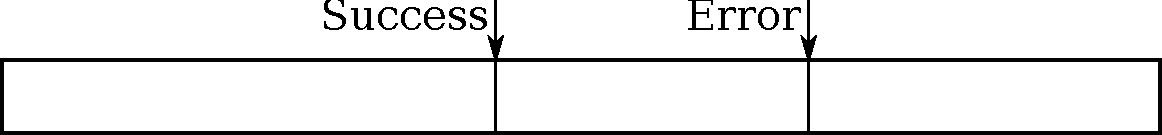
\includegraphics[width=0.75\textwidth]{drawing}
\caption{Illustration of \lstinline{Uncertain}}
\label{fig:uncertain}
\end{figure}

More generally, we can have a situation like the one depicted in 
figure \ref{fig:uncertain}. We have a succesful parse and an error
further ahead. We do not want to throw the error away, because it is
not guarenteed that continuing parsing from the success gets us further
than the error. There are three cases
\begin{enumerate}
\item A successful parse with no errors further ahead
\item A successful parse with errors further ahead
\item No success.
\end{enumerate}
These correspond to the \lstinline{Success}, \lstinline{Uncertain}, and 
\lstinline{Error} constructors respectively. When combining two parses
care must be taken to figure out what type of result the combination
of two things becomes.
[TODO: More detail?]

Note that an
\lstinline{Uncertain} result will eventually turn in to either an
error or a success. Either there will be a successfull result of
parsing all the input in which case there can not be errors further
ahead, or all potential successes (incuding the uncertain ones) will
turn into errors by continued parsing.

\subsection{Precedence and associativity}

With parser combinators the many aspects of the BNF grammar can be
almost directly copied to create the parser. The problems of 
precedence and associativity however requires some care. I will start
by discussing precedence.

Getting precedence to work is a question of making
sure that the parse tree which is used to recognize the string is
a cetain one. That is to unambiguate the grammar. The possible
binary operators are divided into $n$ precedence levels 
from $0$ to $n-1$. The
$\text{op2}_n$ rule regocnizes operators on the $n$th level. Table
\ref{tab:precedence} shows the precedence levels in our implementation.

\begin{table}
\centering
\begin{tabular}{| c | l | }
\hline
0 & $==$, $\neq$ \\
\hline
1 & $<$, $>$, $\leq$, $\geq$ \\
\hline
2 & $:$ \\
\hline
3 & $+$, $-$, $||$ \\
\hline
4 & $*$, $/$, $\%$, $\&\&$ \\
\hline
\end{tabular}
\caption{Precedence levels for the operators in SPL. As it can be seen
 in our case $n=4$, but this is easily extended to any number of
levels}
\label{tab:precedence}
\end{table}

Expressions are divided into $n + 1$ levels. On the $i$th level are 
expressions which are a number of expressions combined by a level
$i$ binary operator. The first of these expressions is a level
$i+1$ expression
and the remaining are level $i$. The $n$th level contains all 
expressions which are not applications of binary operators.
The only one of these which is non trivial is the application of a
unary operator,
since it contains a subexpression, and we have to decide on a
level for this subexpression. Making this a level $n$ expression
causes unary operators to have highest precedence, which is the
desired effect.
That is for $0 \leq i < n$ the grammar looks as
\begin{align*}
\text{exp}_i ::=&\ \text{exp}'_i\ [ \text{op2}_i\ \text{exp}_i ] \\
\text{exp}'_i ::=&\ \text{exp}_{i+1} 
\end{align*}
And for $n$ we have defined:
\begin{align*}
\text{exp}'_{n} ::=&\ \ldots \\
    | &\ \text{op1}\ \text{exp}'_{n} \\
    | &\ \ldots
\end{align*}
Here the dots represent all the non operator expression types.

\section{Type checker}
What are the typing rules?

Probably discuss the inference monad thing, and definitly the whole
substitution show.

Polymorphism of values

missing feature: Type annotations

Our mistake. Throwing away type information.

\section{Code generation}

Code generation is handled by recursively traversing the AST, generating
a list of instructions at each node by pasting together the code
generated by the children and adding relevant extra instructions.

During this traversal some state is kept using a state monad. In
particular we keep track of an integer used to generate unique label
names, and the current variable context, i.e. a map
from variable names to integers representing where they can be found
relative to the base pointer(MP) of the current stack frame.

In addition the function for generating code for an expression node
takes a boolean argument, which will be expanded upon in section
\ref{sec:gc}, and the function for generating code for a statement
node takes a string denoting the label to jump to in the case of a 
return statement.

[TODO: Should we have more about standard code generation?]

\subsection{Stack layout}
One of the key design decicions in code generation is the stack
layout. The SSM has nice instructions for dealing with call stacks
which suggest a certain design. We have mainly used this, but in
order for garbage collection to work we have some extra constraints 
which needs to be handled which complicates the stack layout a little
bit.

\begin{enumerate}
\item At runtime we have to know how many local variables 
including arguments are 
associated with a frame, and where they are.
\item A local can only contain a reference to a heap object if that
heap object is actually alive.
\end{enumerate}
\begin{table}
\centering
\begin{tabular}{l | c |}
  & arg $n$ \\
\cline{2-2}
  & ... \\
\cline{2-2}
  & arg 2 \\
\cline{2-2}
  & arg 1 \\
\cline{2-2}
  & ret. addr.  \\
\cline{2-2}
MP& old MP \\
\cline{2-2}
  & $m+n$ \\
\cline{2-2}
  & local $m$ = 0 \\
\cline{2-2}
  & ... \\
\cline{2-2}
  & local 2 = 0\\
\cline{2-2}
  & local 1 = 0 \\
\cline{2-2}
  & copy of arg 1 \\
\cline{2-2}
  & copy of arg 2 \\
\cline{2-2}
  & ... \\
\cline{2-2}
SP& copy of arg $n$ 
\end{tabular}
\caption{Stack layout after prologue of function has been executed}
\label{tab:stackframe}
\end{table}
Table \ref{tab:stackframe} shows what a stack frame looks like right
after the function prologue has been run. The main differences from
what a stack frame created by a normal \lstinline{bsr funcion} followed
by a \lstinline{link m} is the following:
\begin{enumerate}
\item An extra field containing the total number of locals ($m+n$)
 has been added right after the MP.
\item All arguments have been copied into local variable space.
\item All newly created local variables that are not arguments have
 been zeroed.
\end{enumerate}
The first two points makes sure that the garbage collector can easily
find and traverse through all variables associated with a frame.
The third point makes sure that a local will not accidentially contain
a pointer to some heap structure which is not actually in use.

In the actual body of the function arguments are always obtained
through the copy in local variable space. The arguments supplied by
the caller are not used after they have been copied initially.

\subsection{Pairs and lists}

All basic types, booleans, integers (and void)  are represented by a
single word and passed around to functions as values.

For pairs and lists this will not work, not only do they not fit into
a single word, because they can be nested they can be of arbitrary 
size. Therefore all pairs and lists are allocated on the heap. On
the stack and when passed to functions they are represented by a
reference to their heap object. This reference is also passed by value.

Discussion of the exact structure of a heap object is defered to
section \ref{sec:gc:heap}. For now we just assume the existence of 
a subroutine (not directly accecibly by the programmer) which takes
two words, stores them in a new heap object, and returns a reference
to this new object.

Everytime the syntactical form \lstinline{(X, Y)} is encountered a
new pair is allocated with \lstinline{X} and \lstinline{Y} as data.

Lists are linked lists. This fits the syntax. Creating array semantics
for cons/nil hd/tl style syntax would be cumbersome, and probably end
up with a lot of reallocations and inefficient code in general. This
means that a list can either be nil, which is represented by the value
0 or it can be a cons cell cointaining some data and a next pointer.
Cons cells are treated similarily to pairs.

\subsection{Missing features}

The code generation of our compiler has some missing features. The
two main ones are support for global variables and the overloaded print
function. As mentioned in section \ref{sec:type:missing} due to the
way we designed the type checker we do not actually have type information
at later stages. This is problem when trying to implement overloaded
functions.

In addition labels in the assembly code are not handled super rigoriously.
It might be possible to write code that produces assember with two
identical labels at different places in the code. Also a main function
is required, but that it actually exists is not checked. A branch
instruction to a main label is just inserted after the initial setup
code.

\section{Garbage collection}

As our extension we have chosen to implement garbage collection, so that
memory can be reclaimed without the programmer having to manually free
it. We have implemented a copying garbage collector. It works by splitting 
the heap space into two equally sized parts. Only one of the parts is 
in use at a time. When there is no more space in that part a collection
is initiated. The collection makes the other part of the heap the 
currently active one and then reallocates all heap object from the old
part which are still in use. All references pointing to copied(reallocated)
objects needs to be updated. This removes all heap object to which no
references exists, while completely avoiding fragmentation. The cost is
that the user can only use half of the available memory space (in
virtual memory environments this does not neccesarily imply that not
all actual memory is available).

\subsection{Heap object layout}

All heap object takes up 4 words of memory. Only 3 of these are used,
but we need an even number to keep alignment. The layout is shown
in table \ref{tab:heapobj}. Two words is used for the data. Head and 
tail or first and second depending on wether it is a list or a 
pair. In theory it would be
possible to reduce the size to 2 words since we only need the forwading
pointer when the data does no longer matter.

\begin{table}
\centering
\begin{tabular}{| c |}
\hline
unused \\
\hline
forwarding pointer \\
\hline
data \\
\hline
data \\
\hline
\end{tabular}
\caption{Heap object layout}
\label{tab:heapobj}
\end{table}

When allocating a new object, we need to set the forwarding pointer
such that it is guarenteed to not point the the currently inactive
region of heap memory. In our implementation it points to the beginning
of the heap object, only because that was convenient. It could just
as well have replicated one of the data fields, or been set to a consant
even number.

When allocating it is also checked if there is enough heap space.
If not a collection is initiated.

\subsection{Tagging}

The algorithm, which will be elaborated in more detail later, 
 depends on being able to discern between references and
values at runtime. Since the heap pointer starts at an even address, 
all heap objects have size 4, and references point to the end of heap
objects, every reference will be an odd number. We make sure to multiply
all values by two before storing them to a memory location (and 
dividing them by two again before doing computation with them on the
stack). This process we refer to as tagging (and detagging). In the
case of references tagging and detagging them is simply a no op(In
addition tagging and detaggin the value 0 is also a no op, this is 
important because lists are always either references or 0 in the case
of nil).
This provides a method of discerning values from references, namely
parity. 

Actually realizing this is not completely trivial. Detagging is always
quite easy, because we can use the tag to determince how to detag
\footnote{However we don't actually even have to do this, it turns
out we can completely determine if we are untagging a reference or a 
value at runtime. This will be elaborated later}. Tagging is the more
difficult process because it is not always trivial to see if we are
dealing with references or values. The process of
tagging happens in assignment statements
\begin{lstlisting}
a = X;
\end{lstlisting}
where \lstinline{X} is any kind of expression. It is tempting to 
let all expression code deal exclusively in untagged values (by 
immediatly untagging any value loaded from memory and never tagging
anything) and then
tagging right before assignment, in the statement generating code.
This works in most cases because we know wether the resutl of an 
expression is a reference or a value. However, consider the case where
\lstinline{X} is just a variable. In this case it is not known wether
we are dealing with a reference or a value. To find this out type
information would be needed, but as explained in section \ref{sec:type}
it is not available and making it so seems like a lot of work.

Stepping a bit back, actually storing one variable into another is just
moving a tagged value from one place to another. We should not actually
have to do anything to it, and therefore we should be able to perform
this operation without type information. This is indeed possible, but
it requires the code generation for expressions to be able to work 
with tagged values.

The way we solve this is by having the expression code generation
function taking an argument which specifies wether it should deliver
a tagged or an untagged value on the stack. Pushing conversions down
like this, which allows us to completely avoid them if they are not
needed, turns out to work remarkably well even without type
information.

There is even a trick we can use, exploiting that detagging a reference
is a no op. If we generate code for an expression and we know that it
will result in a reference, we can ask for a tagged value even if we
need an untagged one. Applying this everywhere it turns out that we
can avoid every single situation where untagging a reference would
otherwise be needed. This means that the untagging code simply becomes
division by 2. There is no need to check if we are trying to untag a
reference, because we never are.

\subsection{Cheney's algorithm}

In this section the garbage collection algorithm itself is described
in more detail. Fundamentally it is Cheney's algorithm \cite{cheney}.

They key part is the \emph{forward} operation. The rest of the algorithm
is just about applying this to the right things in the right order.
The forward operation takes a pointer, makes sure the object pointed
to has been reallocated on the new active part of the heap, and then
returns the new location. It works in three steps as described below.

\begin{enumerate}
\item If the input is not a pointer, or already points to new part of
 heap, return the input directly.
\item If the forwarding pointer of the object pointed to by the input
 points to the new part of the memory, return the forwarding pointer.
\item Otherwise reallocate the data, then set the forwarding pointer of
 the old object to the new location. Return the pointer to the new location.
\end{enumerate}

Note that this procedure is not recursive. If a heap object itself
contains pointers, just forwarding it is not enough. We explicitly
want to move all the active objects to the new heap in a breath first
way. This greatly simplifies updating all pointers.

Now for the actual algorithm. The first step is changing which half
of the memory space we use. In order to keep track of our memory three
values, all stored in registers are used. The first is the standard
heap pointer (R3/HP), which tells us where to next allocate memory.
Next the \emph{limit} of the current part of memory is held in R5.
Finally the \emph{other} value in R6 points to the beginning of the
part of memory not currently un use. Also recall that R7 holds to initial
value of MP, which is not a valid stack frame.

\begin{algorithmic}
\State $scan \gets \mathrm{R6}$ \Comment{R6 is other}
\State $\mathrm{R6} \gets \mathrm{R5} - size$ \Comment{R5 is limit}
\State $\mathrm{R5} \gets scan + size$
\State \Comment{Now the active part of the heap is changed, and $scan$ points
to beginning of newly activated part}
\State $base \gets [\mathrm{MP}]$
\While{$base \neq \mathrm{R7}$} \Comment{forward roots}
    \State $i \gets 2$
    \State $locals \gets [base + 1] + 2$
    \While{$i < locals$}
        \State $[base + 1] \gets \mathrm{forward}([base + 1])$
    \EndWhile
    \State $base \gets [base]$
\EndWhile
\While{$scan < \mathrm{HP}$} \Comment{forward rest by bfs}
    \State $[scan + 2] \gets \mathrm{forward}([scan + 2])$
    \State $[scan + 3] \gets \mathrm{forward}([scan + 3])$
    \State $scan \gets scan + 4$
\EndWhile
\end{algorithmic}

This is all implemented in assembler and appended onto every program.

[TODO: Explain algorithm in more detail]

\section{Tests}

\printbibliography


\end{document}
